\documentclass[journal,12pt,onecolumn]{IEEEtran}
\usepackage[utf8]{inputenc}   % Codificación de entrada
\usepackage[T1]{fontenc}      % Codificación de fuente
\usepackage[spanish,es-tabla]{babel}   % Idioma español
\usepackage{lmodern}          % Fuente moderna
\usepackage{amsmath, amssymb} % Matemáticas y símbolos
\usepackage{graphicx} 		  % Gráficos e imágenes
\graphicspath{{img/}{tablas/}{portada/}}  % Las imágenes se buscarán en la carpeta "img"
\usepackage{longtable}      % Para tablas que se extienden en varias páginas
\usepackage{tabularx}	% Tablas avanzadas
\usepackage{threeparttable}
\usepackage{hyperref}	% Hipervínculos

%-------------------------------------------
% Otros paquetes útiles (personaliza según tus necesidades)
%-------------------------------------------
\usepackage{caption}
\usepackage{subcaption}
\usepackage{xcolor}
\usepackage{setspace}

%-------------------------------------------
% Comandos personalizados
\renewcommand{\listtablename}{Índice de tablas}
\renewcommand{\appendixname}{Anexos}
\definecolor{colorreferences}{RGB}{48,134,3}

% Metadatos del PDF
\hypersetup{
	unicode=true,
	hidelinks,
	colorlinks=true,       % false: boxed links; true: colored links
	linkcolor=black,          % color of internal links (change box color with linkbordercolor)
	citecolor=colorreferences,        % color of links to bibliography
	filecolor=magenta,      % color of file links
	urlcolor=blue,           % color of external links
	linkbordercolor={0 0 0}
}
%-------------------------------------------
% Inicio del documento
%-------------------------------------------
\begin{document}

% Aquí se encuentra el archivo con la portada
\begin{titlepage}
	\centering
	%-------------------------------------------
	% Logos en una tabla: izquierda, centro y derecha
	\begin{tabular}{@{}p{0.3\textwidth} p{0.3\textwidth} p{0.3\textwidth}@{}}
		
\includegraphics[height=2cm]{tecnm} & 
		\centering 
\includegraphics[height=1.5cm]{SEP} & 
		\raggedleft 
\includegraphics[height=2cm]{ith.jpg} \\
	\end{tabular}
	
	\vspace{2em}
	
	\noindent
	%-------------------------------------------
	%	Información institucional y académica (esquina superior izquierda)
	\begin{minipage}[t]{0.48\textwidth}
		\raggedright
		\small \textbf{%
			Instituto Tecnológico de Hermosillo\\
			Materia: Robótica\\
			Profesor: Medina Gil Lamadrid, Jesús Iván%
		}
	\end{minipage}%
	\hfill
	%	fecha actual (esquina superior derecha), en letras pequeñas y en negrita.
	\begin{minipage}[t]{0.48\textwidth}
		\raggedleft
		\small \textbf{\today}
	\end{minipage}
	
	\vspace{2em}
	
	%-----------------------------------------
	% Unidad y Título de la tarea en letras grandes y en negrita
	{\large \textbf{Unidad 1: Morfología del robot}}\\
	{\Huge \textbf{Tipos de Sensores}}
		
	\vspace{1em}
	
	%---------------------------------------
	% Tabla con la información del equipo
	%---------------------------------------
	% Encabezado del equipo
	\begin{center}
		{\Large \textbf{Equipo 2}}
	\end{center}
	
	\vspace{1em}
	
	% Tabla de integrantes:
	% Cada fila contiene: foto (columna izquierda) y datos del integrante (columna derecha)
	\begin{center}
		\begin{tabular}{c c}
			\begin{tabular}{c}
				
\includegraphics[height=3cm]{Cedano.jpeg} \\
				\textbf{Cedano Mendoza},\\ Carlos Francisco \\ \texttt{L21330552@hermosillo.tecnm.mx} \\ Teléfono: 6624686707
			\end{tabular} &
			\begin{tabular}{c}
				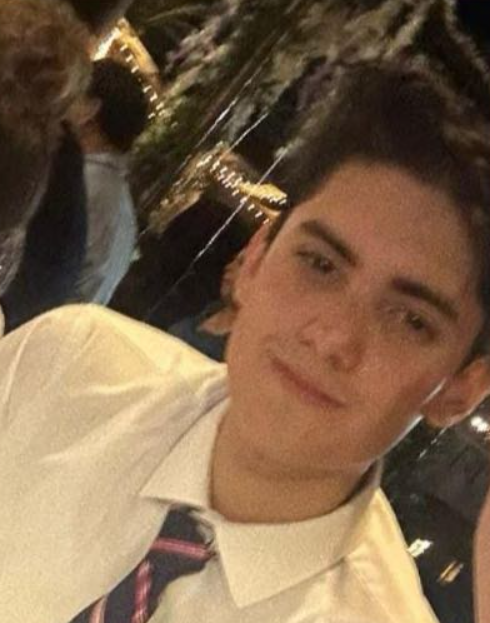
\includegraphics[height=3cm]{Martinez.png} \\
				\textbf{Martinez Navarro,}\\ Sebastian \\ \texttt{L2133} \\ Teléfono: 6621053764
			\end{tabular} \\ \vspace{2em}
			\begin{tabular}{c}
				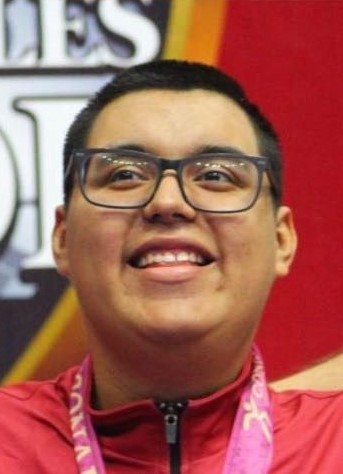
\includegraphics[height=3cm]{Ocampo.jpeg} \\
				\textbf{Ocampo Ramos,}\\ Addiel Adrián \\ \texttt{L20330895@hermosillo.tecnm.mx} \\ Teléfono: 6623501716
			\end{tabular} &
			\begin{tabular}{c}
				\includegraphics[height=3cm]{Pérez.jpeg} \\
				\textbf{Pérez Estupiñán,}\\ Ana Claudia \\ \texttt{L21330669@hermosillo.tecnm.mx} \\ Teléfono: 6624281154
			\end{tabular}
		\end{tabular}
	\end{center}

\end{titlepage}

%	Es innecesario poner el índice porque ya aparece en los marcadores del PDF
%\tableofcontents

% Ejemplo de inclusión de una sección (por ejemplo, "introduccion.tex" debe estar en la carpeta "secciones" y se recomienda no usar carácteres especiales (tilde) o espacios)


\section{Imágenes}
En \LaTeX, las imágenes se pueden incluir utilizando el paquete \texttt{graphicx}. 
Para añadir una imagen en texstudio, es posible arrastrarla directamente en el editor, lo que obtendrá como resultado lo mostrado en la \autoref{fig:insertarimagen}.

\begin{figure}[h]
	\centering
	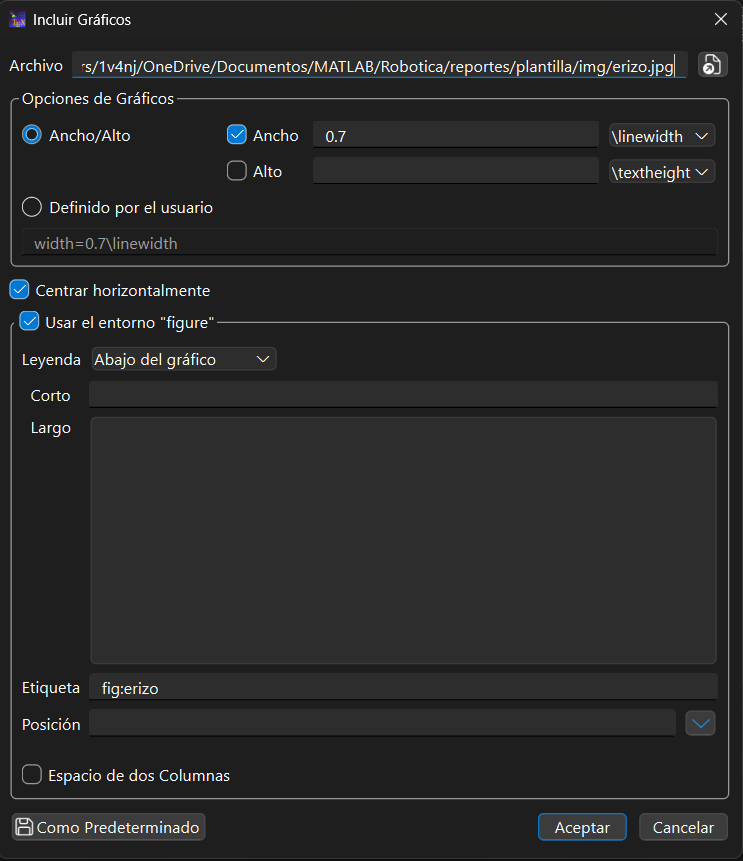
\includegraphics[width=0.7\linewidth]{img/insertarImagen}
	\caption{Opciones al insertar una imagen}
	\label{fig:insertarimagen}
\end{figure}
\cit
Algunas opciones clave incluyen:

\begin{itemize}
	\item \textbf{Tamaño de la imagen}: Se puede definir un ancho o alto relativo a la caja de texto o se puede usar un tamaño en pixeles (px), centímetros (cm) o el ancho de la letra M (em).
	\item \textbf{Centrado}: Se puede marcar la opción para que la imagen aparezca centrada automáticamente.
	\item \textbf{Uso del entorno `figure'}: Permite que la imagen tenga una numeración automática y pueda referenciarse en el texto con \texttt{\textbackslash ref\{\}} o \texttt{\textbackslash autoref\{\}}.
	\item \textbf{Posicionamiento (`h`, `t`, `b`, `p`)}: Al presionar la flecha de la derecha, podemos añadir las opciones que determinan la posición de la imagen en el documento, como después del texto o arriba de la página, etc. Si igual vamos a referenciar las figuras, es innecesario que estén exactamente donde fueron mencionadas ya que eso deja muchos espacios en blanco.
	\item \textbf{Leyenda Largo}: permite poner una descripción de la imagen en el lugar que elegimos (debería de estar debajo).
	\item \textbf{Etiqueta}: nos servirá para referenciarla. 
\end{itemize}

Para usar dos imágenes como en \autoref{fig:mascotas}, se utilizó \texttt{subfloat}.
% Dos imágenes de mascotas
\begin{figure}[h]
	\centering
	\subfloat[Perro]{%
		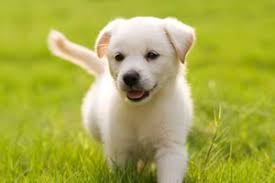
\includegraphics[width=0.4\textwidth]{perro.jpg}%
		\label{fig:perro}
	}
	\hfill
	\subfloat[Gato]{%
		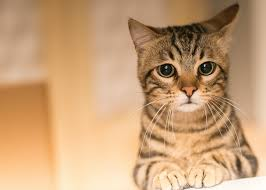
\includegraphics[width=0.4\textwidth]{gato.jpg}%
		\label{fig:gato}
	}
	\caption{Imagen de dos mascotas}
	\label{fig:mascotas}
\end{figure}
\section{Tablas}
Existen varias formas de crear tablas además de este entorno, como \texttt{array}, \texttt{longtable} y \texttt{tabularx}, que permiten manejar datos extensos de manera eficiente. También es posible convertirlas desde páginas, como en \href{https://tableconvert.com/es/excel-to-latex}{TableConvert}, que permite transformar datos de Excel a formato \LaTeX fácilmente.

A continuación, se presenta una tabla larga como ejemplo:

\newcounter{actividad} % Define un contador llamado "actividad"
\begin{longtable}{|c|p{10cm}|c|} % Define anchos específicos
	\caption{Ejemplo de Tabla Larga.} \label{tab:ejemplo_tabla} \\
	\hline
	\textbf{No.} & \textbf{Descripción} & \textbf{Estado} \\
	\hline
	\endfirsthead
	\multicolumn{3}{c}{{\tablename\ \thetable{} -- continuación}} \\
	\hline
	\textbf{No.} & \textbf{Descripción} & \textbf{Estado} \\
	\hline
	\endhead
	\hline \multicolumn{3}{r}{{Continúa en la siguiente página...}} \\
	\hline
	\endfoot
	\hline
	\endlastfoot
	% Contenido de la tabla
	1 & Lorem ipsum dolor sit amet, consectetur adipiscing elit. & Completado \\
	2 & Sed do eiusmod tempor incididunt ut labore et dolore magna aliqua. & En proceso \\
	3 & Ut enim ad minim veniam, quis nostrud exercitation ullamco laboris. & Pendiente \\
	4 & Duis aute irure dolor in reprehenderit in voluptate velit. & Pendiente \\
	5 & Excepteur sint occaecat cupidatat non proident. & Pendiente \\
	6 & Sunt in culpa qui officia deserunt mollit anim id est laborum. & Pendiente \\
	7 & Curabitur pretium tincidunt lacus, nulla gravida orci a odio. & Pendiente \\
	8 & Nullam varius, turpis et commodo pharetra. & Pendiente \\
	9 & Sed ac orci quis tortor imperdiet venenatis. & Pendiente \\
	10 & Duis eget orci sit amet orci dignissim rutrum. & Pendiente \\
	11 & Nam dui ligula, fringilla a, euismod sodales, sollicitudin vel, wisi. & Pendiente \\
	12 & Pellentesque habitant morbi tristique senectus et netus et malesuada. & Pendiente \\
	13 & Fusce convallis metus id felis luctus adipiscing. & Pendiente \\
	14 & Pellentesque dapibus hendrerit tortor. & Pendiente \\
	15 & Praesent egestas tristique nibh. & Pendiente \\
	16 & Curabitur a felis in nunc fringilla tristique. & Pendiente \\
	17 & Phasellus nec sem in justo pellentesque facilisis. & Pendiente \\
	18 & Etiam imperdiet imperdiet orci. & Pendiente \\
	19 & Vestibulum ante ipsum primis in faucibus orci luctus et ultrices. & Pendiente \\
	20 & Quisque id mi. Integer ante arcu, accumsan a, consectetuer eget, posuere ut, mauris. & Pendiente \\
\end{longtable}
\section{Ecuaciones}
Para realizar ecuaciones, se pueden ayudar mucho de ChatGPT (Como copiar una imagen y que lea la ecuación para dártela en formato \LaTeX) y de que MATLAB, word y algunas páginas te permiten copiar ecuaciones en formato \LaTeX. El modelo en espacio de estados de un robot de dos grados de libertad, el cual se puede ver en el Capítulo 5: Dinámica del Robot en \cite{barrientos2007fundamentos} se expresa como

\begin{equation}
	\label{eq:spaceStateRobot}
	\begin{bmatrix}
		\dot{q} \\
		\ddot{q}
	\end{bmatrix} =
	\begin{bmatrix}
		0 & I \\
		M^{-1}(-C - G)
	\end{bmatrix}
	\begin{bmatrix}
		q \\
		\dot{q}
	\end{bmatrix} +
	\begin{bmatrix}
		0 \\
		M^{-1} B
	\end{bmatrix} u,
\end{equation}
donde:
\begin{itemize}
	\item \( q \) es el vector de posiciones articulares del robot.
	\item \( \dot{q} \) y \( \ddot{q} \) son las velocidades y aceleraciones articulares.
	\item \( M \) es la matriz de inercia.
	\item \( C \) representa las fuerzas centrífugas y de Coriolis.
	\item \( G \) es el vector de fuerzas gravitacionales.
	\item \( B \) es la matriz de entrada de los torques.
	\item \( u \) es el vector de torques aplicados a las articulaciones.
\end{itemize}

Cabe destacar que en \eqref{eq:spaceStateRobot}, la ecuación se referencia después de haberla nombrado y forma parte de la oración, por lo que debe llevar puntos o comas. También al referenciar, debe de estar entre paréntesis con \texttt{eqref}.
\section{Conclusión}
En la elaboración de este reporte, se utilizó por primera vez el software LaTeX para la edición del documento y Sourcetree para la gestión del control de movimientos entre modificaciones de datos del documento por parte de los distintos miembros del equipo. A lo largo del proceso, se presentaron dificultades relacionadas con el uso de Sourcetree, especialmente en la ejecución de comandos como branches, commit, push y pull, lo que requirió una curva de aprendizaje adicional para comprender su funcionamiento y evitar conflictos en la sincronización de archivos.

A pesar de estos desafíos, la experiencia permitió familiarizarse con herramientas clave para la edición y gestión colaborativa de documentos, lo que resultará beneficioso en futuros proyectos. La combinación de LaTeX y Sourcetree demostró ser una opción robusta para la elaboración de reportes técnicos con un control de organización eficiente, aunque es recomendable seguir profundizando en su uso para optimizar los flujos de trabajo y minimizar errores.

Por otra parte, el conocimiento más importante obtenido de la investigación sobre los distintos tipos de sensores fue la comprensión de cómo cada tecnología responde a necesidades específicas en diversas industrias. Esta investigación permitió no solo identificar las aplicaciones clave de cada sensor, sino también comprender la importancia de la selección adecuada según el entorno y el tipo de medición requerida. La evolución de los sensores, junto con su integración con inteligencia artificial y procesamiento de datos, sigue impulsando innovaciones en automatización, control y análisis del entorno.









%-------------------------------------------
% Bibliografía
%-------------------------------------------
\bibliographystyle{IEEEtran}  % Estilo de bibliografía IEEE
% La bibliografía se tomará del archivo "fuentes.bib"
\bibliography{fuentes}
	
\end{document}
